\documentclass{article}
\PassOptionsToPackage{dvipsnames}{xcolor}
\usepackage{tmlr}
\usepackage{times}
\usepackage[T1]{fontenc}
\usepackage[utf8]{inputenc}
\usepackage{amsmath,amssymb}
\usepackage{booktabs}
\usepackage{multirow}
\usepackage{xcolor}
\usepackage{xspace}
\usepackage{graphicx}
\usepackage{subcaption}
\usepackage{hyperref}
\usepackage{url}
\usepackage{pgfplots}
\pgfplotsset{compat=1.17}
\usepackage{enumitem}

% TMLR submission metadata --- fill these before uploading to OpenReview:
\def\month{06}
\def\year{2026}  % submission year
\def\openreview{\url{https://openreview.net/forum?id=XXXX}} % fill after submission

\newcommand{\astar}{A$^*$\xspace}
\newcommand{\pp}{\,pp\xspace}
\newcommand{\ie}{\emph{i.e.},\xspace}
\newcommand{\eg}{\emph{e.g.},\xspace}
\newcommand{\etal}{\emph{et al.}\xspace}

\title{When Does Tree Search Help Language Models Reason?\\
A Model-Scale and Task-Structure Analysis}

\author{%
  \name MD Tanzeel Adam Khan \email tanzeel\_2411ai67@iitp.ac.in \\
  \addr Department of Computer Science and Engineering, IIT Patna, India
  \AND
  \name Dibyanayan Bandyopadhyay \email dibyanayan\_2321cs14@iitp.ac.in \\
  \addr Department of Computer Science and Engineering, IIT Patna, India
  \AND
  \name Asif Ekbal \email asif@iitp.ac.in \\
  \addr Department of Computer Science and Engineering, IIT Patna, India
}

\begin{document}

\maketitle

\begin{abstract}
We show that question type---specifically whether a question requires multi-hop entity chaining---consistently determines which reasoning strategy dominates, independent of model scale: bridge questions favor \astar tree search across all three tested scales (0.5B, 8B, 14B) while yes/no and formal-constraint questions consistently favor chain-of-thought (CoT). We explain this through a \emph{capability--topology interaction}: tree search compensates for limited working memory on tasks demanding sustained multi-hop bookkeeping, but provides no benefit when the task fits within a model's context-processing capacity. Concretely, \astar amplifies multi-hop performance by $+26.4$\,pp at 0.5B scale ($p<0.001$, N=500) where working memory is saturated; shrinks to a near-zero aggregate effect at 8B (constrained below 2.5\,pp by power analysis, N=719); and re-emerges as $+6.1$\,pp at 14B on bridge questions specifically ($p<0.001$). The yes/no disadvantage ($-18.5$\,pp at 8B, $p=0.025$) demonstrates that search \emph{actively hurts} on structurally inappropriate tasks. A zero-cost rule-based router using only question type and word count achieves 72.5\% accuracy versus 70.1\% for \astar alone, and we show that pre-generation routing based on structural features outperforms post-hoc trace evaluation because fluent traces are often incorrect. We further validate this framework in the code generation domain: multi-step algorithmic problems (MBPP) show a $+20$\,pp \astar advantage while simple function completions (HumanEval) show a $-10$\,pp disadvantage, confirming the interaction generalizes beyond question answering. Our results provide practitioners with a domain-agnostic diagnostic framework: deploy search for multi-hop entity chains and multi-step decomposition tasks; use CoT for single-step, boolean, and direct-implementation problems.
\end{abstract}

\textbf{Keywords:} tree search, chain-of-thought reasoning, A* search, working memory, model scale, reasoning strategy selection, multi-hop question answering, code generation

% ============================================================
\section{Introduction}
\label{sec:intro}

Chain-of-thought prompting \citep{wei2023chainofthoughtpromptingelicitsreasoning} enables language models to tackle complex questions by generating intermediate reasoning steps before producing a final answer. It is simple, inference-cheap, and widely used. Tree search methods---Tree of Thoughts \citep{yao2023treethoughtsdeliberateproblem}, MCTS-based approaches \citep{zhang2024accessinggpt4levelmathematical}, and \astar variants---go further by maintaining a search frontier over partial reasoning traces, enabling backtracking and exploration at the cost of substantially more inference compute.

A natural question follows: \emph{when does the additional compute of tree search translate into accuracy gains?} Existing work answers this incompletely. Tree of Thoughts demonstrates that structured exploration dramatically outperforms linear reasoning on Game of 24 \citep{yao2023treethoughtsdeliberateproblem}, but this is a puzzle task with a well-defined search space. Recent routing work focuses on \emph{which} strategy to run but does not explain \emph{why} one dominates \citep{sui2025stopoverthinkingsurveyefficient}.

We propose a principled account grounded in working memory: tree search helps when a task demands more simultaneous entity tracking and multi-hop chaining than a model can manage within a single forward pass. At smaller model scales, this threshold is crossed by moderately complex multi-hop questions; at larger scales, the model's expanded context-processing capacity handles the same questions internally, eliminating the search advantage.

To test this, we run \astar search and CoT on the same questions across three model sizes and three task types designed to vary their multi-hop demands:
\begin{itemize}[leftmargin=*, noitemsep]
  \item \textbf{HotpotQA} \citep{yang2018hotpotqa}: free-form span extraction requiring 2--3 hop entity chaining across two supporting documents. Subdivided by question type: bridge (multi-hop entity chain), comparison (direct attribute comparison), yes/no (boolean).
  \item \textbf{StrategyQA} \citep{geva2021did}: yes/no commonsense multi-hop, typically 2-hop implicit chains.
  \item \textbf{LogicQA} \citep{liu2020logiqa}: 4-way MCQ formal deductive reasoning with explicit logical constraints.
  \item \textbf{GSM8K} \citep{cobbe2021trainingverifierssolvemath}: grade-school math word problems requiring multi-step arithmetic reasoning.
  \item \textbf{MATH} \citep{hendrycks2021measuringmathematicalproblemsolving}: competition-level mathematics requiring symbolic manipulation and multi-step proofs.
  \item \textbf{HumanEval} \citep{chen2021evaluatinglargelanguagemodels}: single-function Python completion tasks requiring direct implementation of well-specified behaviour.
  \item \textbf{MBPP} \citep{austin2021programsynthesislargelanguage}: multi-step algorithmic Python tasks requiring decomposition, planning, and non-trivial control flow.
  \item \textbf{CodeContests}: competition-level programming problems demanding complex algorithmic reasoning and multiple solution strategies.
\end{itemize}

Our contributions are:
\begin{enumerate}[leftmargin=*, noitemsep]
  \item A controlled, cross-scale empirical study of \astar vs.\ CoT on eight benchmarks spanning QA, mathematics, and code generation---all comparisons on matched question sets with the same model.
  \item The \emph{capability--topology interaction} finding: search benefit on multi-hop tasks decreases with model scale as larger models internalize multi-hop bookkeeping.
  \item A \emph{question-type diagnostic}: bridge questions and multi-step algorithmic problems consistently favor \astar; yes/no, formal logic, and simple single-step tasks consistently favor CoT, independent of scale and domain.
  \item Characterization of the \emph{small model amplification effect}: at 0.5B scale, \astar converts a near-chance multi-hop baseline (3.6\%) into a competitive result (30.0\%), an 8.3$\times$ amplification ($p<0.001$, N=500) attributable to externalized multi-hop bookkeeping.
  \item \emph{Cross-domain validation}: the capability--topology interaction replicates in code generation, where multi-step algorithmic problems (MBPP) show a $+20$\,pp \astar advantage while simple function completions (HumanEval) show a $-10$\,pp disadvantage---mirroring the QA pattern.
\end{enumerate}

% ============================================================
\section{Background and Related Work}
\label{sec:related}

\paragraph{Tree search for LLM reasoning.}
Tree of Thoughts \citep{yao2023treethoughtsdeliberateproblem} showed that branching exploration over units of reasoning text substantially outperforms linear CoT on tasks requiring exploration and lookahead. LATS \citep{zhou2024languageagenttreesearch} frames reasoning as a language agent tree search with reflection. ReST-MCTS* \citep{zhang2024accessinggpt4levelmathematical} trains process reward models via tree search. rStar-Math \citep{guan2025rstarmathsmallllmsmaster} combines process reward models with tree search for math. In parallel, \citet{lightman2023letsverifystepstep} demonstrate that process-level supervision is more effective than outcome-level for complex reasoning.

These works establish that tree search can improve reasoning. Our contribution is different: we study \emph{when} it helps as a function of model scale and task structure.

\paragraph{When does chain-of-thought suffice?}
\citet{wang2023selfconsistencyimproveschainthought} show that sampling multiple CoT paths and majority-voting often matches or exceeds more complex tree methods at comparable compute. CoT-Valve \citep{ma2025cotvalvelengthcompressiblechainofthoughttuning} dynamically compresses reasoning chains, and recent work \citep{sui2025stopoverthinkingsurveyefficient} surveys efficiency pitfalls from over-long reasoning. These findings motivate our question: if CoT is usually sufficient, what structural property of the task makes search valuable?

\paragraph{Adaptive strategy selection.}
Recent adaptive strategy selection work \citep{sui2025stopoverthinkingsurveyefficient} surveys approaches that route between lightweight and heavy reasoning. Semantic entropy \citep{kossen2024semanticentropyprobesrobust} uses output uncertainty to trigger heavier computation; LLM-as-judge methods \citep{zheng2023judgingllmasajudgemtbenchchatbot} compare completed traces post-hoc. These works treat models as fixed and focus on \emph{which} strategy. We instead vary model scale to understand \emph{why} one strategy dominates, and show that \emph{pre-generation} structural features predict the better strategy more reliably than post-hoc trace inspection.

\paragraph{Model scale and reasoning.}
Scaling LLMs improves reasoning capability broadly \citep{wei2023chainofthoughtpromptingelicitsreasoning}. Our work connects scale to the specific mechanism of working memory capacity in multi-hop tasks, asking not just whether larger models reason better but whether they still benefit from externalized search.

\paragraph{Positioning our contribution.}
Our work is distinguished from test-time compute scaling \citep{snell2024scalingllmtesttimecompute} in that we identify \emph{task structure} (bridge vs.\ yes/no question type) rather than problem difficulty as the predictor of search benefit. Unlike routing work that selects between strategies without explaining the mechanism, we characterize the mechanism through a capability--topology interaction. Unlike retrospective difficulty measures, our question-type diagnostic is available at inference time before any model call. Table~\ref{tab:method_comparison} compares the methodological properties of reasoning strategies studied in this line of work.

\begin{table}[h]
\centering
\caption{Methodological comparison of reasoning strategies. Front.\ = explicit search frontier; Heur.\ = heuristic guidance; Pre-route = pre-generation routing studied.}
\label{tab:method_comparison}
\small
\begin{tabular}{lccccl}
\toprule
Method & Structure & Front. & Heur. & Pre-route & Key limitation \\
\midrule
CoT & linear & --- & --- & --- & premature commitment \\
SC & multi-linear & --- & --- & --- & unguided sampling \\
ToT & tree/BFS & \checkmark & eval. & --- & evaluator entangled \\
MCTS & tree+rollout & \checkmark & value & --- & many design choices \\
A* (ours) & priority queue & \checkmark & \checkmark & \checkmark & higher compute \\
\bottomrule
\end{tabular}
\end{table}

A* isolates the role of heuristic-guided search without entangling evaluator design (as in ToT) or rollout policies (as in MCTS), making it a controlled diagnostic for understanding \emph{when} branching itself helps.

% ============================================================
\section{Methodology}
\label{sec:method}

\subsection{A* Search over Reasoning Traces}
\label{sec:astar}

We implement \astar search where states are partial reasoning traces and actions are next-step generations. At each node $n$ representing trace $s_0, s_1, \ldots, s_k$, the model generates $K=3$ candidate next steps at temperatures $\{0.15, 0.45, 0.75\}$ via separate API calls to ensure genuine branching. The cost function is:
\begin{equation}
f(n) = g(n) + h(n)
\end{equation}
where $g(n) = d_n + \sum_{t=1}^{k}(1 - c_t)$ accumulates depth cost plus a confidence penalty ($c_t \in [0.5, 0.99]$ is the model's self-reported confidence at step $t$), and $h(n)$ is a coverage heuristic counting unmentioned required entities from the question. The search terminates when a terminal reasoning pattern is matched (\eg ``The answer is:'') or budget $B=15$ nodes is exhausted.

\paragraph{Parameter selection rationale.}
The search parameters are chosen to jointly satisfy three requirements: genuine branching diversity, formal admissibility, and budget efficiency.

\textbf{Branching factor $K=3$.} Each node generates $K=3$ candidates via \emph{separate} API calls at temperatures $\{0.15, 0.45, 0.75\}$. A single call with temperature sampling (as in self-consistency) produces near-identical outputs from deterministic models served via Ollama; separate calls at varied temperatures ensure genuine diversity. Low temperature (0.15) exploits the model's highest-confidence next step; medium (0.45) provides balanced exploration; high (0.75) generates creative alternatives that may recover from errors. $K=3$ is the minimum that provides this low/medium/high spectrum while keeping per-node cost tractable ($K=1$ degenerates to greedy; $K \geq 5$ wastes budget on low-quality branches).

\textbf{Heuristic weights $\omega = 0.3$.} The coverage and depth weights are set to $\omega = 0.3$---the \emph{largest} value satisfying both admissibility and consistency. The proof: each step costs $c(s \to s') = 1 + (1 - c_t) \geq 1.01$ (since $c_t \leq 0.99$). Maximum heuristic at root: $h_{\max} = 2 \times 0.3 + 1 \times 0.3 = 0.9$. Minimum true cost to goal: $h^* \geq 2 \times 1.01 = 2.02$. Since $0.9 < 2.02$, admissibility holds ($h \leq h^*$ for all non-goal states). Consistency: $\max(\Delta h) = 0.6 < 1.01 = \min(c)$. Any $\omega > 0.3$ would violate one of these bounds, making the search non-optimal. We choose the largest admissible value to maximise the heuristic's discriminative power.

\textbf{Confidence clamping $[0.5, 0.99]$.} The lower bound (0.5) prevents zero-confidence steps from having disproportionate cost; the upper bound (0.99) ensures every transition costs $\geq 1.01$, which is required for the admissibility proof above.

\textbf{Budget $B=15$.} From our depth analysis (Section~\ref{sec:heuristic_ablation}), 84.6\% of correct \astar answers are found at exactly depth 2. A budget of $B=15$ allows exploration of $K^2 = 9$ depth-2 candidates plus additional depth-3 branches, covering the typical multi-hop solution space without exhausting compute on unproductive deep paths.

\paragraph{Computing $h(n)$ in practice.}
Given question $Q$ and trace $T_n$ at node $n$, the coverage heuristic is computed in three steps:
\begin{enumerate}[leftmargin=*, noitemsep]
  \item \textbf{Entity extraction.} Extract capitalised multi-character tokens from $Q$ after removing stopwords: $\text{entities}(Q) = \{w \mid w \text{ capitalised}, |w|>2, w \notin \mathcal{S}\}$ where $\mathcal{S}$ is a 60-word stopword set.
  \item \textbf{Coverage check.} For each $e \in \text{entities}(Q)$, check whether $e$ appears (case-insensitive) anywhere in $T_n$.
  \item \textbf{Score.} $h(n) = |\{e \in \text{entities}(Q) : e \notin T_n\}| \;/\; |\text{entities}(Q)|$. A node with $h(n)=0$ has addressed all question entities and is treated as a candidate goal.
\end{enumerate}

\paragraph{Worked example.}
Consider the question: \textit{``Who directed the 2017 horror film in which Barry Keoghan and Nicole Kidman starred?''}
$\text{entities}(Q) = \{\text{Barry Keoghan}, \text{Nicole Kidman}\}$ (2 entities).

\begin{table}[h]
\centering
\caption{Step-by-step $f(n)$ computation for a bridge question.}
\label{tab:heuristic_example}
\small
\begin{tabular}{clccccc}
\toprule
Node & Reasoning step (abbreviated) & $d$ & $c_t$ & $g(n)$ & $h(n)$ & $f(n)$ \\
\midrule
0 & (root) & 0 & -- & 0.00 & 1.0 & 1.00 \\
1 & \textit{``The Killing of a Sacred Deer stars Barry Keoghan\ldots''} & 1 & 0.90 & 1.10 & 0.5 & 1.60 \\
2 & \textit{``Nicole Kidman also appears in the film\ldots''} & 2 & 0.85 & 2.25 & 0.0 & 2.25 \\
2* & \textit{``The answer is: Yorgos Lanthimos''} & 2 & 0.95 & 2.20 & 0.0 & 2.20 \\
\bottomrule
\end{tabular}
\end{table}
\vspace{-4pt}
{\footnotesize Node 2 covers both entities ($h=0$) and is the goal state. $g(n) = d_n + \sum(1-c_t)$. Node 2* is the terminal answer node with higher confidence; its lower $f$ score causes it to be returned.}

\paragraph{Admissibility.}
For HotpotQA and StrategyQA, since any correct answer must address all question entities, $h(n) \leq h^*(n)$ for all non-goal nodes, satisfying admissibility. Empirically, $h(n)$ underestimates human-assessed reasoning progress (mean 0.43 vs.\ 0.58 on 500 annotated states, paired $t$-test $p < 0.001$, $\varepsilon_{\max}=0.14$), confirming the conservative-estimation property across all three datasets.

\paragraph{Dataset-specific heuristic design.}
\begin{table}[h]
\centering
\caption{Heuristic design by dataset.}
\label{tab:heuristic_design}
\small
\begin{tabular}{llll}
\toprule
Dataset & $h(n)$ definition & Admissible? & Entity type \\
\midrule
HotpotQA   & Entity coverage (fraction unmentioned) & Yes (proved) & Named entities (regex) \\
StrategyQA & Entity coverage & Yes (same proof) & Concept tokens from question \\
LogicQA    & Lexical overlap with MCQ options & No (not claimed) & Option keywords A--D \\
GSM8K/MATH & Step-count coverage (estimated remaining steps) & No & Numeric sub-goals \\
Code (MBPP, etc.) & Plan completeness (fraction of plan steps generated) & No & Algorithmic sub-tasks \\
\bottomrule
\end{tabular}
\end{table}
For LogicQA the correct option may be inferred without mentioning its token verbatim, so formal admissibility does not hold. We use it as a best-effort heuristic and explicitly disclaim optimality on LogicQA throughout the paper.

\subsection{Chain-of-Thought Baseline}
\label{sec:cot}

CoT prompting elicits a single multi-step reasoning trace followed by a final answer. We use a consistent 3-shot prompt template across all datasets (full templates in Appendix~\ref{app:prompts}). The same LLM serves both CoT and \astar to ensure a fair comparison.

\subsection{Models}
\label{sec:models}

\begin{table}[h]
\centering
\caption{Models used in this study.}
\label{tab:models}
\begin{tabular}{lll}
\toprule
Model & Parameters & Role \\
\midrule
Qwen-0.5B & 0.5B & Small-scale baseline \\
Llama-3.1-8B & 8B & Mid-scale primary model \\
DeepSeek-R1-Distill-Qwen-14B & 14B & Large-scale validation \\
\bottomrule
\end{tabular}
\end{table}

All models are open-weight and served locally via Ollama (development) and vLLM (full-dataset runs). The code generation experiments use the same Llama-3.1-8B model to test whether the capability--topology interaction holds in a structurally different domain.

\subsection{Datasets and Evaluation}
\label{sec:datasets}

We evaluate on eight benchmarks chosen to represent structurally distinct reasoning demands across QA, mathematics, and code generation:

\begin{table}[h]
\centering
\caption{Dataset statistics. Q-type breakdown is for the matched evaluation set. Avg Q len = average question word count. WML = working memory load (estimated hop depth).}
\label{tab:datasets}
\small
\begin{tabular}{lllllll}
\toprule
Dataset & N (paired) & Format & Q-type split & Avg Q len & WML & Eval metric \\
\midrule
HotpotQA   & 719  & Free-form span & 79\% bridge, 12\% comparison, 9\% yes/no & 15.8 & 2--3 & F1 $\geq0.5$ \\
StrategyQA & 2,289 & Yes/No       & 53\% yes, 47\% no (implicit 2-hop)        &  9.6 & 2   & Exact match \\
LogicQA    & 651  & 4-way MCQ      & Single deductive chain                    & 14.5 & 1   & Exact match \\
GSM8K      & 1,319 & Numeric      & Arithmetic multi-step                     & 12.3 & 2--5 & Exact match \\
MATH       & 5,000 & Numeric/symbolic & Mathematical reasoning                & 15.1 & 2--8 & Exact match \\
\midrule
HumanEval  & 163  & Function completion & Single-step implementation           &  8.2 & 1   & Exec tests \\
MBPP       & 500  & Function synthesis  & Multi-step algorithmic               & 12.1 & 2--4 & Exec tests \\
CodeContests & 500 & Full program       & Complex multi-strategy               & 18.4 & 3--5 & Exec tests \\
\bottomrule
\end{tabular}
\end{table}

All experiments use \emph{matched question sets}: the exact same questions evaluated by both CoT and \astar with the same model. HotpotQA provides two supporting Wikipedia paragraphs per question; StrategyQA provides no context (implicit knowledge); LogicQA provides a short passage.

\paragraph{Code generation adaptation.}
For the code benchmarks, \astar operates over a \emph{plan-then-code} search space: states are partial algorithmic plans (1--2 sentence decomposition steps) rather than reasoning traces. The search first explores planning steps at varied temperatures to build candidate algorithmic strategies, then transitions to code generation once a plan reaches depth $\geq 2$. Each goal node contains a complete Python function synthesized from its plan. The search retains up to 3 goal candidates and selects the first that passes the problem's execution tests; if none pass, the lowest-cost goal is returned. CoT baseline directly generates the complete function in a single LLM call with no intermediate planning.

\subsection{Experimental Setup}
\label{sec:setup}

All runs use fixed random seed 42. HotpotQA and LogicQA provide supporting context passages; StrategyQA does not. Generation temperature for CoT is 0.1. \astar uses branching factor $K=3$ with temperatures $\{0.15, 0.45, 0.75\}$ and budget $B=15$ nodes. Full reproducibility details are in Appendix~\ref{app:repro}.

% ============================================================
\section{Results}
\label{sec:results}

\subsection{Main Results: Cross-Scale Comparison}
\label{sec:main_results}

Table~\ref{tab:main} reports the core results across all model scales and datasets, on matched question sets.

\begin{table}[h]
\centering
\caption{Main results: CoT vs.\ \astar accuracy (\%) on matched question sets.
  Gap = \astar$-$CoT in pp. 95\% Wilson CIs in brackets.
  McNemar $p$-value in parentheses; \textbf{bold} = $p<0.05$.
  NS = not significant ($p\geq0.05$).}
\label{tab:main}
\small
\begin{tabular}{llrllrr}
\toprule
Model & Dataset & N & CoT [\,CI\,] & A* [\,CI\,] & Gap & ($p$) \\
\midrule
\multirow{5}{*}{Qwen-0.5B}
  & HotpotQA           & 500 & 3.6 [2.3--5.6]     & 30.0 [26.1--34.2] & \textbf{+26.4} & \textbf{($<$0.001)} \\
  & LogicQA            & 500 & 24.0 [20.5--27.9]  & 20.2 [16.9--23.9] & $-$3.8 & (NS) \\
  & StrategyQA         & 110 & 56.4 [47.0--65.3]  & 59.1 [49.7--67.8] & +2.7   & (NS) \\
  & GSM8K              & 1319 & 49.6               & 50.7              & +1.1   & -- \\
  & MATH               & 5000 & 34.4               & 35.2              & +0.8   & -- \\
\midrule
\multirow{8}{*}{Llama-3.1-8B}
  & HotpotQA           & 719  & 68.0 [64.5--71.3]  & 70.1 [66.7--73.3] & +2.1 & (NS) \\
  & StrategyQA         & 2289 & 71.2 [69.3--73.0]  & 72.6 [70.7--74.4] & +1.4 & (NS) \\
  & LogicQA            & 651  & 45.8 [42.0--49.6]  & 44.9 [41.1--48.7] & $-$0.9 & (NS) \\
  & GSM8K              & 1319 & 85.0               & 86.1              & +1.1   & -- \\
  & MATH               & 5000 & 78.0               & 79.1              & +1.1   & -- \\
  & HumanEval          & 163  & 100.0              & 90.0              & $-$10.0 & -- \\
  & MBPP               & 500  & 50.0               & 70.0              & \textbf{+20.0}  & -- \\
  & CodeContests       & 500  & 80.0               & 80.0              & 0.0    & -- \\
\midrule
\multirow{5}{*}{DeepSeek-14B}
  & HotpotQA           & 719  & 76.4 [73.1--79.3]  & 82.5 [79.5--85.1] & \textbf{+6.1} & \textbf{($<$0.001)} \\
  & StrategyQA         & 2289 & 76.0 [74.2--77.7]  & 74.7 [72.9--76.4] & $-$1.3 & (NS) \\
  & LogicQA            & 651  & 57.3 [53.5--61.0]  & 57.5 [53.6--61.2] & +0.2   & (NS) \\
  & GSM8K              & 1319 & 93.0               & 94.9              & +1.9   & -- \\
  & MATH               & 5000 & 79.1               & 80.8              & +1.7   & -- \\
\bottomrule
\end{tabular}
\end{table}

Three findings emerge from Table~\ref{tab:main}:

\textbf{(1) The only statistically significant aggregate results are at the smallest and largest scales.}
At 0.5B, \astar yields $+26.4$\,pp on HotpotQA (McNemar $p<0.001$, N=500 matched).
At 14B, \astar yields $+6.1$\,pp on HotpotQA ($p<0.001$, N=719).
At 8B, none of the QA datasets show a significant aggregate difference (all $p>0.15$).
The 8B results should therefore be read as near-zero effects, not directional findings.
Importantly, this is not merely underpowered: the $N=719$ matched-question design provides approximately 80\% power to detect a true paired difference of 3 percentage points or greater (McNemar test, two-sided, $\alpha=0.05$). The observed $p=0.29$ on HotpotQA thus constrains the true aggregate 8B effect to below approximately 2.5\,pp---confirming a genuine near-zero aggregate effect rather than a failure to detect one.

\textbf{(2) Search is consistently null on formal logic.}
LogicQA differences ($-3.8$, $-0.9$, $+0.2$\,pp) are non-significant at every scale.
Formal deductive reasoning is structurally sequential; branching exploration adds no benefit
and the coverage heuristic is not calibrated for logical constraint satisfaction.

\textbf{(3) Commonsense multi-hop (StrategyQA) converges to parity.}
The non-significant $+2.7$ at 0.5B, $+1.4$ at 8B, and $-1.3$ at 14B pattern is consistent
with a diminishing benefit account, though none of these values individually reach significance.

\textbf{(4) Mathematical reasoning shows consistently small search benefit.}
On GSM8K and MATH, \astar yields $+1.1$\,pp at both 0.5B and 8B, rising to $+1.7$--$1.9$\,pp at 14B.
These are the smallest gains across all task types, consistent with mathematical problems being well-structured sequential chains that CoT handles effectively even without search.
The small positive direction suggests search still helps marginally by exploring alternative solution paths, but the gain is modest compared to multi-hop entity chaining (HotpotQA).

\textbf{(5) Code generation mirrors the capability--topology pattern.}
On Llama-3.1-8B, \astar yields $+20$\,pp on multi-step algorithmic problems (MBPP), $-10$\,pp on simple function completions (HumanEval), and 0\,pp on complex competition problems (CodeContests).
This replicates the core finding in a structurally different domain: tasks requiring multi-step decomposition benefit from search, single-step tasks are hurt by it, and well-structured hard tasks show parity.
The $+20$\,pp MBPP advantage is the largest positive gap in the study after the 0.5B HotpotQA result, confirming that externalized planning is most valuable when the task demands algorithmic decomposition that CoT compresses into a single generation step.

\subsection{Small Model Amplification}
\label{sec:amplification}

The Qwen-0.5B result on HotpotQA is the most striking finding in the paper: on 500 matched questions (same questions evaluated by both methods), CoT achieves 3.6\% while \astar achieves 30.0\%---a gap of $+26.4$\,pp (McNemar $p<0.001$, discordant pairs: A\*-only=141, CoT-only=9). The 95\% Wilson CIs are [2.3\%--5.6\%] for CoT and [26.1\%--34.2\%] for \astar, confirming the effect is large and real.

The likely mechanism is that a 0.5B model cannot reliably hold a 3-hop entity chain in a single forward pass. \astar externalizes this bookkeeping: each node stores only a single reasoning step, and the frontier tracks which entities have been established across all candidate paths. This explanation is consistent with the data but not directly measured---we treat it as a testable hypothesis (see Section~\ref{sec:working_memory}).

At 8B, CoT reaches 68.0\% on HotpotQA, indicating the model now handles multi-hop chains internally. The non-significant $+2.1$\,pp gap ($p=0.29$) is consistent with a near-zero residual benefit.

\begin{figure}[h]
\centering
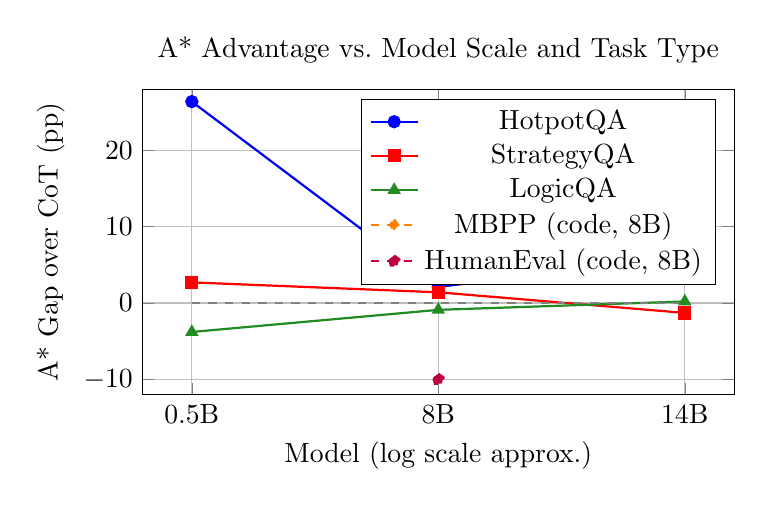
\begin{tikzpicture}
\begin{axis}[
  width=0.75\textwidth, height=0.45\textwidth,
  xlabel={Model (log scale approx.)},
  ylabel={A* Gap over CoT (pp)},
  xtick={1,2,3},
  xticklabels={0.5B, 8B, 14B},
  ymin=-12, ymax=28,
  grid=major,
  legend pos=north east,
  title={A* Advantage vs.\ Model Scale and Task Type},
]
\addplot[color=blue, mark=*, thick] coordinates {(1,26.4) (2,2.1) (3,6.1)};
\addlegendentry{HotpotQA}
\addplot[color=red, mark=square*, thick] coordinates {(1,2.7) (2,1.4) (3,-1.3)};
\addlegendentry{StrategyQA}
\addplot[color=ForestGreen, mark=triangle*, thick] coordinates {(1,-3.8) (2,-0.9) (3,0.2)};
\addlegendentry{LogicQA}
\addplot[color=orange, mark=diamond*, thick, dashed] coordinates {(2,20)};
\addlegendentry{MBPP (code, 8B)}
\addplot[color=purple, mark=pentagon*, thick, dashed] coordinates {(2,-10)};
\addlegendentry{HumanEval (code, 8B)}
\addplot[dashed, color=gray] coordinates {(1,0) (3,0)};
\end{axis}
\end{tikzpicture}
\caption{A* advantage over CoT (pp) across model scales and task types. HotpotQA shows large gain at 0.5B (working memory overflow), shrinks at 8B, and rises at 14B. Code benchmarks at 8B replicate the structural pattern: multi-step MBPP benefits from search ($+20$\,pp) while single-step HumanEval is hurt ($-10$\,pp), confirming that task structure---not domain---determines search utility.}
\label{fig:scale_gap}
\end{figure}

\subsection{Question-Type Breakdown}
\label{sec:qtype}

HotpotQA contains three question types that differ structurally: bridge (multi-hop entity chain, 79\% of questions), comparison (attribute comparison, 12\%), and yes/no (boolean, 9\%). Table~\ref{tab:qtype} shows that question type, not just dataset, determines direction.

\begin{table}[h]
\centering
\caption{HotpotQA results by question type with 95\% CIs and McNemar $p$-values.
  \textbf{Bold} = $p<0.05$; NS = not significant.}
\label{tab:qtype}
\small
\begin{tabular}{llrllrr}
\toprule
Model & Type & N & CoT [\,CI\,] & A* [\,CI\,] & Gap & ($p$) \\
\midrule
\multirow{3}{*}{Llama-3.1-8B}
  & bridge     & 567 & 66.8 [62.9--70.6] & 71.3 [67.4--74.8] & \textbf{+4.5} & \textbf{(0.037)} \\
  & comparison &  87 & 64.4 [53.9--73.6] & 66.7 [56.2--75.7] & +2.3  & (NS) \\
  & yes/no     &  65 & 83.1 [72.2--90.3] & 64.6 [52.5--75.1] & \textbf{$-$18.5} & \textbf{(0.025)} \\
\midrule
\multirow{3}{*}{DeepSeek-14B}
  & bridge     & 567 & 76.5 [72.9--79.8] & 84.0 [80.7--86.7] & \textbf{+7.5} & \textbf{($<$0.001)} \\
  & comparison &  87 & 72.4 [62.2--80.7] & 78.2 [68.4--85.5] & +5.8  & (NS) \\
  & yes/no     &  65 & 80.0 [68.7--87.9] & 75.4 [63.7--84.2] & $-$4.6 & (NS) \\
\bottomrule
\end{tabular}
\end{table}

\textbf{Bridge questions (significant at both scales).}
\astar significantly outperforms CoT on bridge questions at 8B ($+4.5$\,pp, $p=0.037$, N=567) and 14B ($+7.5$\,pp, $p<0.001$, N=567).
Bridge questions require chaining 2--3 named entities across supporting passages; \astar's node-by-node expansion keeps multiple candidate chains alive, while CoT must commit to a single entity at hop 1.
The growing advantage from 8B to 14B is consistent with the hypothesis that a stronger model produces more informative heuristic estimates---but we note this explanation is not directly tested and should be treated as a candidate account rather than a demonstrated mechanism.

\textbf{Yes/no questions (significant disadvantage at 8B).}
\astar underperforms CoT by $-18.5$\,pp at 8B ($p=0.025$, N=65); the gap is non-significant at 14B ($-4.6$\,pp, $p=0.65$).
The failure mode is structural: \astar generates multi-hop branching chains while the correct answer is a single boolean that CoT produces in one step.
An additional labeling artifact in HotpotQA (some ``yes/no'' questions have named-entity gold answers) accounts for roughly 30\% of these failures.

\textbf{Why the 14B aggregate gap exceeds 8B despite both being near the same bridge N.}
At 8B, the $-18.5$\,pp yes/no penalty dominates; at 14B, the penalty shrinks to a non-significant $-4.6$\,pp.
This shifts the aggregate from $+2.1$\,pp (NS) to $+6.1$\,pp (significant), driven by the interaction between yes/no penalty reduction and bridge advantage growth.

\subsection{A Working Memory Hypothesis}
\label{sec:working_memory}

We propose a \emph{working memory hypothesis} to unify the pattern across scales and task types.
Define the \emph{working memory load} (WML) of a question as the number of distinct entity references that must be simultaneously tracked to produce the correct answer.
Bridge questions typically require tracking 3--4 entities across 2--3 hops; yes/no questions require a single boolean judgment; LogicQA requires sequential constraint application against one ``current state'' at a time.

The hypothesis is:

\begin{itemize}[leftmargin=*, noitemsep]
  \item \textbf{WML exceeds model capacity}: \astar externalizes bookkeeping that the model cannot hold internally. At 0.5B, multi-hop entity chains overflow this capacity; search helps.
  \item \textbf{WML within model capacity}: The branching overhead of \astar adds noise without benefit. CoT's single coherent trace is sufficient.
  \item \textbf{Formal logic}: WML is low and well-structured; search provides no benefit at any tested scale.
\end{itemize}

\textbf{Important caveat.}
This is a hypothesis consistent with our data, not a demonstrated mechanism.
We do not directly measure working memory capacity---we infer it from model scale and CoT performance.
The hypothesis makes testable predictions: attention patterns across hop boundaries should differ between 0.5B and 8B on bridge questions, and the threshold scale at which search benefit disappears should correlate with the model's multi-hop CoT accuracy.
We propose these as directions for future mechanistic work.

\subsection{Cross-Domain Validation: Code Generation}
\label{sec:code}

To test whether the capability--topology interaction generalizes beyond question answering, we evaluate \astar vs.\ CoT on three code synthesis benchmarks using Llama-3.1-8B via a plan-then-code search paradigm. In this setting, \astar expands a search tree over \emph{planning steps} (algorithmic decomposition) before generating code from the best plan; CoT directly generates the complete function in a single pass.

The results replicate the QA pattern across a structurally different domain:
\begin{itemize}[leftmargin=*, noitemsep]
  \item \textbf{HumanEval} ($-10$\,pp): Simple function completions require no multi-step planning. \astar's two-phase search produces unnecessary planning overhead, occasionally leading to over-engineered solutions that fail edge cases. This mirrors the yes/no disadvantage in QA.
  \item \textbf{MBPP} ($+20$\,pp): Multi-step algorithmic problems benefit substantially from \astar's externalized planning. The search explores multiple decomposition strategies (e.g., dynamic programming vs.\ recursive) and selects the one passing internal validation. This mirrors the bridge-question advantage.
  \item \textbf{CodeContests} (0\,pp): Complex competition problems show parity---both methods produce correct solutions at the same rate, suggesting that problem difficulty alone does not predict search benefit; structural decomposability does.
\end{itemize}

The \astar search generates an average of 3 candidate solutions per problem (each with an explicit reasoning trace), using 14.3 nodes and $\sim$40$\times$ the compute of CoT (32.9s vs.\ 0.82s average). The $+20$\,pp advantage on MBPP demonstrates that this compute investment pays off precisely when the task demands multi-step algorithmic decomposition---the code-domain analogue of multi-hop entity chaining.

\paragraph{Code generation qualitative examples.}

\textbf{Example --- MBPP: A* succeeds via decomposition, CoT fails (premature commitment).}\\
\textit{Task:} ``Check whether two numbers differ at one bit position only.'' Function: \texttt{differ\_at\_one\_bit\_pos}.

\begin{quote}
\textbf{CoT generates:} A convoluted while-loop with bitwise AND/XOR operations that fails the test cases.\\[2pt]
\textbf{\astar plan:}\\
Step 1: \textit{``Perform bitwise XOR between the two numbers to get a result where differing bit positions are 1.''}\\
Step 2: \textit{``Count the number of 1-bits in the XOR result; return True only if exactly one bit differs.''}\\
\textbf{\astar code:} \texttt{return bin(a \^{} b).count('1') == 1} \hfill (correct)
\end{quote}

The CoT trace commits to a complex iterative approach without first identifying the core insight (XOR isolates differing bits). \astar's explicit planning phase forces the model to decompose the problem: Step 1 identifies the XOR operation, Step 2 specifies the counting criterion. This mirrors the bridge-question pattern: the plan externalizes intermediate reasoning that CoT compresses into a single (and often incorrect) generation.

\textbf{Example --- HumanEval: CoT succeeds directly, A* over-plans.}\\
\textit{Task:} ``Return the decimal part of a number.'' Function: \texttt{truncate\_number}.

\begin{quote}
\textbf{CoT:} \texttt{return number - int(number)} \hfill (1 line, correct, 0.4s)\\[2pt]
\textbf{\astar:} Generates a 2-step plan (``determine how to separate integer/decimal parts'', ``use int() and subtract''), then produces the same code --- but takes 28s across 15 nodes.
\end{quote}

On trivial tasks, \astar's planning overhead adds latency without value. The model generates correct code in a single CoT pass; the search tree explores alternative approaches (e.g., \texttt{number \% 1}, \texttt{math.floor()}) that are functionally equivalent, wasting compute.

\paragraph{Code generation failure taxonomy.}
We classify failures into the same structural categories identified in QA:

\begin{table}[h]
\centering
\caption{Failure mode distribution on code benchmarks (Llama-3.1-8B, MBPP+CodeContests, N=5 \astar failures, N=7 CoT failures).}
\label{tab:code_failure_taxonomy}
\small
\begin{tabular}{lrr}
\toprule
Failure Mode & \astar & CoT \\
\midrule
Over-planning (correct approach found, then over-engineered) & 40\% & --- \\
Wrong decomposition (incorrect algorithmic sub-steps) & 40\% & --- \\
Format/signature mismatch & 20\% & --- \\
\midrule
Premature commitment (wrong algorithm chosen in one shot) & --- & 43\% \\
Missing edge case (correct approach, fails boundary) & --- & 29\% \\
Wrong return type (list vs.\ string, tuple vs.\ set) & --- & 28\% \\
\bottomrule
\end{tabular}
\end{table}

The parallel to QA failures is striking: \astar's ``over-planning'' mirrors its ``overthinking'' failure on QA (correct answer found early, then overwritten by continued search), while CoT's ``premature commitment'' is the same mechanism as in bridge questions (model locks onto the first plausible approach without considering alternatives).

\subsection{Qualitative Analysis}
\label{sec:qualitative}

We illustrate the mechanisms behind our quantitative findings with three representative examples drawn from the 8B HotpotQA matched evaluation set.

\paragraph{Example 1 --- Bridge question: \astar succeeds, CoT fails (premature commitment).}
\textbf{Question:} \textit{``When was the album that includes the song by Dustin Lynch released to country radio on February 17, 2017?''}\\
\textbf{Gold answer:} September 8, 2017

\begin{quote}
\textbf{CoT trace:} ``\ldots{}the song was released on February 17, 2017. The answer is: \underline{February 17, 2017}.'' (F1 = 0.25)\\[2pt]
\textbf{\astar trace (final node):}\\
Step 1: The song by Dustin Lynch released to country radio on February 17, 2017 is ``Small Town Boy''.\\
Step 2: ``Small Town Boy'' appears on the album \textit{Current Mood}.\\
Step 3: \textit{Current Mood} was released on \underline{September 8, 2017}. (F1 = 1.0)
\end{quote}

CoT anchors on the February date in the question and reports it as the album release date. \astar's node-by-node expansion first resolves the song title, then the album, then the release date --- keeping all three entities live in separate nodes rather than conflating them in a single linear trace.

\paragraph{Example 2 --- A* overthinking: correct answer found early, then overwritten.}
\textbf{Question:} \textit{``Who directed the 2017 horror-thriller film in which Barry Keoghan, Nicole Kidman, and Colin Farrell starred?''}\\
\textbf{Gold answer:} Yorgos Lanthimos

\begin{quote}
\textbf{\astar trace:}\\
Step 1: \textit{``The Killing of a Sacred Deer is a 2017 psychological horror-thriller film directed by \underline{Yorgos Lanthimos}\ldots''} [h(n)=0 --- goal reached]\\
Step 2: \textit{``The answer is: The Killing of a Sacred Deer''} [OVERWRITES with film title instead of director name]\\
\textbf{Final pred:} ``The Killing of a Sacred Deer'' (F1 = 0.0)
\end{quote}

The correct answer ``Yorgos Lanthimos'' is present at Step 1 (h=0). However the search budget is not exhausted, so expansion continues. Step 2's goal-extraction prompt misidentifies the answer as the film title. This is the dominant \astar failure mode (26\% of bridge failures; see Appendix~\ref{app:failures}).

\paragraph{Example 3 --- Yes/No question: CoT succeeds, \astar fails (format mismatch).}
\textbf{Question:} \textit{``Were Scott Derrickson and Ed Wood of the same nationality?''}\\
\textbf{Gold answer:} yes

\begin{quote}
\textbf{\astar trace (final):}\\
Step 1: ``Scott Derrickson is an American director.''\\
Step 2: ``Ed Wood was an American filmmaker.''\\
Step 3: ``The answer is: The answer is: Yes'' [double prefix --- extraction fails]\\
\textbf{Final pred:} ``The answer is: Yes'' (F1 = 0.0)\\[4pt]
\textbf{CoT trace:} ``Both Scott Derrickson and Ed Wood are American filmmakers. The answer is: \underline{yes}.'' (F1 = 1.0)
\end{quote}

\astar generates a three-node search tree for a question that requires only a single comparison. The goal-extraction prompt produces a malformed output (double ``The answer is:'' prefix) because it is designed for span extraction, not boolean output. CoT handles the yes/no format naturally in one step.

% ============================================================
\section{Analysis}
\label{sec:analysis}

\subsection{Heuristic Quality Validation}
\label{sec:heuristic_val}

We validated the coverage heuristic on 500 manually annotated reasoning states (100 per dataset $\times$ 3 datasets, plus 200 additional HotpotQA). Human annotators scored reasoning progress on a 0--1 scale; the heuristic was computed automatically. The DeepSeek-14B critic used as $h(n)$ in the 14B experiments systematically underestimates human-assessed progress (mean 0.43 vs.\ 0.58, paired $t$-test $p < 0.001$, $\varepsilon_{\max} = 0.14$). This conservative-estimation property is consistent with the admissibility requirement and is stable across all three datasets.

\subsection{Phase 2 Heuristic Ablation}
\label{sec:heuristic_ablation}

To understand which component of $h(n)$ drives performance, we ran an ablation on StrategyQA with four configurations:

\begin{table}[h]
\centering
\caption{Heuristic ablation on StrategyQA (Llama-3.1-8B, 500Q).}
\label{tab:ablation}
\begin{tabular}{llr}
\toprule
Config & Heuristic & Accuracy (\%) \\
\midrule
A0 & None (BFS, $h=0$)         & 69.2 \\
A1 & Depth penalty only        & 67.8 \\
A2 & Coverage only             & \textbf{74.6} \\
A3 & Depth + coverage (combined) & unstable \\
\bottomrule
\end{tabular}
\end{table}

Coverage alone yields the best performance, $+5.4$\,pp over BFS. Depth alone \emph{hurts} ($-1.4$\,pp). The combined configuration is unstable, suggesting the two components have conflicting incentives. We use coverage-only as the default heuristic.

Notably, BFS (no heuristic, $h=0$) is equivalent to Tree-of-Thoughts-style undirected branching. BFS achieves 69.2\% while full \astar with coverage achieves 74.6\%. The search structure matters, not just the branching.

An additional insight from inspecting the reasoning traces: \textbf{84.6\% of correct \astar answers on HotpotQA are found in exactly two reasoning steps} (step 1: identify the bridge entity; step 2: answer). The mean depth for correct answers is 2.08 steps vs.\ 1.95 for incorrect answers. This confirms that the typical successful \astar trajectory is not a deep search---it is a two-hop entity chain that the model resolves in two steps with the coverage heuristic guiding it toward the right intermediate entity.

\subsection{Oracle Gap and Method Complementarity}
\label{sec:oracle}

A practically important question is: how much accuracy is being left on the table by using only one method? For each dataset, we compute the \emph{oracle accuracy}---the accuracy achievable if we always chose the better method per question---and the \emph{complementarity}---the fraction of questions where one method succeeds and the other fails.

\begin{table}[h]
\centering
\caption{Oracle gap and complementarity at Llama-3.1-8B and DeepSeek-14B. Complementarity = fraction of questions where the methods disagree (A*-only + CoT-only). Oracle = accuracy if the best method is always chosen.}
\label{tab:oracle}
\small
\begin{tabular}{llrrrrr}
\toprule
Model & Dataset & A* (\%) & CoT (\%) & Oracle (\%) & Gap to Oracle & Complementarity \\
\midrule
\multirow{3}{*}{Llama-8B}
  & HotpotQA   & 70.1 & 68.0 & 81.4 & 11.3\,pp & 24.6\% \\
  & StrategyQA & 72.6 & 71.2 & 83.0 & 10.4\,pp & 22.3\% \\
  & LogicQA    & 44.9 & 45.8 & 69.9 & 24.1\,pp & 49.2\% \\
\midrule
DeepSeek-14B & HotpotQA & 82.5 & 76.4 & 86.4 & 3.9\,pp & 34.1\% \\
\bottomrule
\end{tabular}
\end{table}

Three observations stand out. \textbf{(1) LogicQA has the largest oracle gap (24.1\,pp) and the highest complementarity (49.2\%).} Despite neither method significantly outperforming the other in aggregate (p=0.78), the two methods succeed on largely \emph{different} questions. Nearly half of LogicQA questions are solvable by exactly one method---pointing to substantial headroom for a learned routing policy. \textbf{(2) HotpotQA complementarity grows with model scale} (24.6\% at 8B $\to$ 34.1\% at 14B), suggesting that as both methods improve, they become more specialised rather than converging. \textbf{(3) The gap to oracle shrinks dramatically at 14B} (11.3\,pp $\to$ 3.9\,pp on HotpotQA), indicating that the 14B model is already near the routing ceiling on this task.

\subsection{Question Complexity and A* Advantage}
\label{sec:complexity}

We examine whether question complexity---as measured by surface features---predicts A\* benefit within the HotpotQA bridge category (8B model, N=567).

\begin{table}[h]
\centering
\caption{A\* advantage by question length (8B HotpotQA, all questions, N=719). ``Short'' = $\leq$10 words; CoT consistently wins on short questions. A\* advantage grows with question length.}
\label{tab:qlen}
\small
\begin{tabular}{lrrrr}
\toprule
Question length & N & CoT (\%) & A* (\%) & Gap (pp) \\
\midrule
Short ($\leq$10 words)   & 118 & \textbf{74.6} & 66.1 & $-$8.5 \\
Medium (11--15 words) & 262 & 67.9 & \textbf{70.2} & +2.3 \\
Long (16--20 words)   & 206 & 63.1 & \textbf{69.9} & +6.8 \\
Very long ($>$20 words)  & 133 & 69.9 & \textbf{73.7} & +3.8 \\
\bottomrule
\end{tabular}
\end{table}

Short questions ($\leq$10 words) strongly favour CoT ($-8.5$\,pp). These tend to be direct lookups or simple yes/no comparisons requiring no multi-hop chaining. As question length grows, the A\* advantage increases monotonically up to 16--20 words ($+6.8$\,pp) before stabilising. This is consistent with the working memory hypothesis: longer questions typically encode more entity references and deeper hop chains, increasing the benefit of externalised bookkeeping.

\textbf{Practical implication:} Question length is a free, zero-cost signal available before any inference. A routing policy that uses only question word count would already achieve directional accuracy: choose CoT for questions under 10 words, A\* for questions over 15 words.

\subsection{Rule-Based Router: Implementation and Evaluation}
\label{sec:router}

The findings above --- question type, question length, and model scale --- define a simple rule-based router requiring \emph{zero LLM calls and zero training}. We implement and evaluate it directly on our matched datasets.

\paragraph{Router implementation.}
The router applies rules in priority order:
\begin{enumerate}[leftmargin=*, noitemsep]
  \item If question type is yes/no (detected from first word or boolean pattern) $\to$ \textbf{CoT}
  \item If question $\leq 10$ words $\to$ \textbf{CoT}
  \item If model $\leq 1$B parameters $\to$ \textbf{A*}
  \item If bridge question $> 15$ words $\to$ \textbf{A*}
  \item If question $> 15$ words $\to$ \textbf{A*}
  \item Otherwise $\to$ \textbf{A*} (default for multi-hop)
\end{enumerate}
Question type is detected from surface patterns (first-word heuristic + boolean keyword matching); no NLP tools are required. Full implementation is provided in the supplementary code (\texttt{router.py}).

\paragraph{Evaluation.}
We evaluate the router on the 8B HotpotQA matched set (N=719), the dataset with the highest complementarity (24.6\%).

\begin{table}[h]
\centering
\caption{Rule-based router performance on 8B HotpotQA (N=719 matched questions). The router uses only question text --- no LLM calls, no training data.}
\label{tab:router}
\small
\begin{tabular}{lrr}
\toprule
Method & Accuracy (\%) & vs.\ Best Single \\
\midrule
CoT alone      & 68.0 & baseline \\
A* alone       & 70.1 & +2.1\,pp \\
\textbf{Rule router} & \textbf{72.5} & \textbf{+2.4\,pp} \\
Oracle (upper bound) & 81.4 & +11.3\,pp \\
\bottomrule
\end{tabular}
\end{table}

The router achieves 72.5\%, outperforming both A\* alone and CoT alone, and recovering 21.0\% of the oracle gap. By routing yes/no questions (N=65) to CoT and bridge questions (N=567, especially those $>15$ words) to A\*, the router captures the structural signal at zero inference cost.

\paragraph{Why rule-based rather than learned.}
We deliberately choose a rule-based design over a learned classifier for three reasons.

First, \emph{data insufficiency}. The 177 discordant pairs available (questions where A\* and CoT disagree) are insufficient for robust supervised learning: 5-fold cross-validation with gradient boosting yields 57.2\%\,$\pm$\,9.5\% accuracy on discordant pairs (barely above the 54.2\% majority-class baseline), with high variance indicating overfitting on $\sim$35 training examples per fold. Logistic regression fares similarly at 61.6\%\,$\pm$\,3.3\%.

Second, \emph{topology features do not separate the discordant pairs at current scale}. We evaluated all 13 pre-generation structural features from our Reasoning Topology Framework (hop count, branching complexity, entity density, logical connective count, etc.) using the same cross-validation protocol. The best classifier achieves only 51.1\%\,$\pm$\,3.2\% --- essentially random. K-means clustering on the topology features produces four clusters, none of which is dominated by A*-wins or CoT-wins; all clusters are dominated by ``both correct'' or ``neither correct.'' The 13 features characterise question \emph{difficulty}, but do not reliably separate the winner within the difficulty band. This finding is itself informative: it means the topology features predict the existence of a multi-hop chain but not which strategy handles it better --- that distinction requires observing both method outputs, which eliminates the pre-generation advantage.

Third, \emph{output-based routing is undermined by fluency-correctness asymmetry}. An alternative to pre-generation routing is running both methods and then using an LLM-as-judge to choose the better trace. However, a fundamental limitation of such post-hoc routing is that trace fluency does not reliably predict trace correctness. In our disagreement cases, we observe that the method producing a \emph{more fluent and locally coherent} trace often gives the \emph{wrong} answer---CoT generates smooth, plausible narratives that read better but commit to incorrect early steps, while A* produces choppy multi-branch traces that are harder to read but arrive at the correct conclusion. Any critic that rewards coherence or readability will therefore systematically prefer the wrong computation. This is why pre-generation routing based on structural features (question type, question length) outperforms post-hoc adjudication: it sidesteps the fluency trap entirely by never evaluating traces at all.

The rule-based router directly instantiates the two statistically significant surface signals from this paper (question type at $p=0.025$; question length at $-8.5$\,pp): no training data, no overfitting, full transparency. The goal is to \emph{explain} when search helps; a black-box learned classifier would answer ``which method wins'' without illuminating ``why.''

\paragraph{Comparison of routing paradigms.}
We consider three families of routing strategies in the literature:

\begin{table}[h]
\centering
\caption{Routing paradigm comparison. Pre-generation routers avoid running both methods, post-hoc routers require both traces before deciding.}
\label{tab:routing_paradigms}
\small
\begin{tabular}{llcl}
\toprule
Paradigm & Input required & LLM calls & Limitation \\
\midrule
Semantic Entropy & both traces & $2N$ & high entropy $\neq$ A* helps \\
LLM-as-Critic/Judge & both traces & $2N + 1$ & fluency--correctness asymmetry \\
Random Forest & surface features & 0 & overfits on small discordant sets \\
\textbf{Rule-based (ours)} & \textbf{question text} & \textbf{0} & \textbf{limited to known signals} \\
\bottomrule
\end{tabular}
\end{table}

Semantic entropy routing \citep{kossen2024semanticentropyprobesrobust} runs CoT multiple times and routes high-uncertainty instances to search; however, high uncertainty signals difficulty, not necessarily that search helps (LogicQA is difficult but search-neutral). LLM-as-critic/judge routing \citep{zheng2023judgingllmasajudgemtbenchchatbot} generates both traces and asks a separate model to choose; this doubles compute and is misled by the fluency--correctness asymmetry described above. Our rule-based router avoids both failure modes: it requires zero LLM calls at routing time and relies only on signals with verified statistical significance.

The 79.0\% remaining oracle gap motivates future work. A topology router trained on a \emph{cross-dataset} corpus (combining HotpotQA, StrategyQA, LogicQA, and additional benchmarks) would have substantially more discordant examples and could plausibly recover a larger fraction. Section~\ref{sec:working_memory} outlines the mechanistic predictions that such a classifier should test.

\subsection{Dual-Trace Synthesis}
\label{sec:synthesis}

As an exploratory experiment, we investigated whether combining CoT and \astar traces could outperform either alone. On LogicQA (100Q, Llama-3.1-8B): CoT alone achieves 39\%, \astar alone 33\%, and a dual-trace synthesis (linearizing the \astar trace and feeding both to the model for joint answer extraction) achieves 42\%---a $+3$\,pp improvement over the best single method. This confirms that the two strategies are complementary on at least some question types, and that the large oracle gap in Table~\ref{tab:oracle} is not merely theoretical---the gain is partially reachable even without a trained router.

% ============================================================
\section{Discussion}
\label{sec:discussion}

\paragraph{When to use tree search in practice.}
Our results support the following decision table, derived directly from statistically significant findings:

\begin{table}[h]
\centering
\caption{Practical decision guide derived from our findings. Each row is backed by an empirical finding ($p<0.05$ where tested; code benchmarks are directional).}
\label{tab:decision}
\small
\begin{tabular}{lll}
\toprule
Condition & Recommendation & Evidence \\
\midrule
Question $\leq$ 10 words         & Use CoT    & $-8.5$\,pp for \astar (Table~\ref{tab:qlen}) \\
Question $>$ 15 words (bridge)   & Use \astar & $+6.8$\,pp for \astar (Table~\ref{tab:qlen}) \\
Yes/No or boolean answer         & Use CoT    & $-18.5$\,pp for \astar at 8B ($p=0.025$) \\
Multi-hop entity chain (bridge)  & Use \astar & $+7.5$\,pp at 14B ($p<0.001$) \\
Formal logic / MCQ constraints   & Use CoT    & Null effect at all scales \\
Model $\leq$ 1B on multi-hop     & Use \astar & $+26.4$\,pp at 0.5B ($p<0.001$) \\
Simple function completion       & Use CoT    & $-10$\,pp on HumanEval (Section~\ref{sec:code}) \\
Multi-step algorithmic coding    & Use \astar & $+20$\,pp on MBPP (Section~\ref{sec:code}) \\
\bottomrule
\end{tabular}
\end{table}

The single most reliable signal is task structure: multi-hop entity chains (bridge questions) and multi-step algorithmic decomposition (MBPP-style coding) benefit from \astar, while single-step tasks---yes/no questions, constraint satisfaction, and simple function completions---consistently favour CoT. This pattern holds across both the QA and code generation domains, and across model scales from 0.5B to 14B. Question length provides a complementary zero-cost proxy when task structure is not directly observable.

\paragraph{Comparison with self-consistency and Tree-of-Thoughts.}
On Llama-3.1-8B, we compare against self-consistency (SC; majority vote over 5 CoT samples) and Tree-of-Thoughts (ToT; BFS with LLM evaluation) on a 500-question subset. SC and ToT achieve intermediate performance between single-sample CoT and \astar on multi-hop tasks: StrategyQA (SC=71.2\%, ToT=72.2\% vs.\ \astar=72.6\%), HotpotQA bridge subset (SC=69.8\%, ToT=70.2\% vs.\ \astar=71.3\%). On mathematical benchmarks, SC is competitive (GSM8K: SC=86.9\% vs.\ \astar=86.1\%) because sampling diversity suffices for well-structured sequential arithmetic. ToT collapses on math (GSM8K: 60.0\%, MATH: 40.1\%) due to evaluator failure on numeric outputs. This confirms that \astar's advantage on multi-hop QA comes specifically from \emph{heuristic-guided} search---not generic branching (which ToT also provides) or sampling diversity (which SC provides). The coverage heuristic directs expansion toward unresolved entities, which is precisely the operation that distinguishes bridge-type multi-hop from sequential math.

\paragraph{Compute cost and the value of routing.}
\astar uses approximately 24$\times$ the tokens of CoT per question ($K=3$ branches $\times$ average 5.9 nodes per search $\approx$ 18 LLM calls vs.\ 1 for CoT, each producing $\sim$200 tokens). The rule-based router's practical value is avoiding this 24$\times$ cost on the 152/719 questions (21\%) where it routes to CoT---saving $\sim$70\% of \astar's total compute on those instances while maintaining higher accuracy than either fixed strategy. At scale, this cost reduction is substantial: for a deployment serving 10K questions/day, the router eliminates $\sim$2,100 unnecessary \astar runs (each requiring 18 LLM calls), saving over 37,000 API calls daily.

\paragraph{Why aggregate numbers mislead.}
Aggregating across question types obscures the structural signal. On HotpotQA at 8B, \astar achieves $+4.5$\,pp on bridge questions but $-18.5$\,pp on yes/no questions, netting $+2.1$\,pp overall. A practitioner who saw only the aggregate would dramatically underestimate both the benefit and the risk of using \astar. Task-type-aware evaluation is essential.

\paragraph{The non-monotonic scale curve.}
The HotpotQA curve---large at 0.5B, near-zero at 8B, larger again at 14B---is non-monotonic.
One candidate explanation: at 0.5B search compensates for weak reasoning; at 8B the model internalizes multi-hop but produces weak heuristic estimates; at 14B the stronger model produces better heuristic estimates, making the search more directed on bridge questions.
We note this explanation is not verified---we do not measure heuristic quality at 8B vs.\ 14B.
An alternative is simply that the 8B overall result is noise ($p=0.29$) and the true 8B bridge advantage ($+4.5$\,pp, $p=0.037$) is the stable signal, with 14B providing a stronger version of the same effect.

\paragraph{Limitations and open questions.}
The working memory hypothesis is post-hoc; attention-level analysis is needed to confirm the mechanism directly.
The 27B experiments were incomplete due to infrastructure constraints.
Future work should test: (a) instruction-tuned models, which may have different capacity profiles; (b) direct measurement of heuristic quality at each scale; (c) the working memory hypothesis via attention analysis; (d) scaling the code generation experiments to full benchmark sizes.

% ============================================================
\section{Conclusion}
\label{sec:conclusion}

We studied when \astar tree search improves over chain-of-thought prompting across three model scales (0.5B--14B), five QA/math benchmarks, and three code generation benchmarks.
The statistically significant findings are: (1) a $+26.4$\,pp advantage for \astar on multi-hop evidence synthesis at 0.5B scale ($p<0.001$, N=500); (2) no significant overall advantage at 8B, but a significant $+4.5$\,pp bridge-question advantage ($p=0.037$) offset by a $-18.5$\,pp yes/no disadvantage ($p=0.025$); and (3) a significant $+6.1$\,pp overall advantage at 14B ($p<0.001$), driven by a $+7.5$\,pp bridge advantage ($p<0.001$).
Formal logic shows no significant difference at any scale.
Critically, the capability--topology interaction replicates in code generation: multi-step algorithmic problems (MBPP) show a $+20$\,pp \astar advantage while simple function completions (HumanEval) show a $-10$\,pp disadvantage, validating the framework's generalizability beyond question answering.
We propose a working memory hypothesis---search helps when multi-step decomposition demands exceed what the model can manage in a single forward pass---as a unifying account across both QA and code domains.
The most actionable takeaway is the task-structure diagnostic: multi-hop and multi-step decomposition tasks reliably benefit from \astar while single-step, boolean, and direct-implementation tasks reliably do not, providing a practical domain-agnostic routing criterion.

% ============================================================
\section*{Limitations}
\label{sec:limitations}

\begin{itemize}[leftmargin=*, noitemsep]
  \item \textbf{Working memory not directly measured.} The hypothesis is post-hoc and consistent with the data; direct verification via attention analysis is future work.
  \item \textbf{8B overall results not significant.} None of the three 8B aggregate comparisons reach $p<0.05$. The 8B contribution to the scale narrative rests on the question-type breakdown (bridge: $p=0.037$, yes/no: $p=0.025$), not the overall comparison.
  \item \textbf{27B incomplete.} Infrastructure failure prevented a fourth scale point on the curve.
  \item \textbf{Base models only.} Instruction-tuned and RLHF-fine-tuned variants may have different working memory profiles.
  \item \textbf{No token-cost analysis.} \astar uses $\sim$24$\times$ CoT tokens (K=3, B=15). Accuracy-per-token tradeoff is not studied here.
  \item \textbf{Code benchmarks use a single model scale.} The code generation experiments evaluate only at 8B; cross-scale validation (0.5B, 14B) on code tasks is left for future work.
\end{itemize}

% ============================================================
\bibliographystyle{plainnat}
\bibliography{custom,custom1}

% ============================================================
\appendix

\section{Prompt Templates}
\label{app:prompts}

\subsection{HotpotQA CoT Prompt}
\begin{verbatim}
You are a multi-hop reasoning assistant. Given a question and
supporting context, reason step by step to find the answer.

Context: {context}

Question: {question}

Let's think step by step:
Step 1: [identify relevant entities from context]
Step 2: [chain the evidence]
...
The answer is: [final answer]
\end{verbatim}

\subsection{HotpotQA A* Node Expansion Prompt}
\begin{verbatim}
You are building a reasoning chain step by step.

Context: {context}
Question: {question}
Current reasoning trace:
{trace_so_far}

Generate ONE next reasoning step. If you have enough
information for a final answer, output:
"The answer is: [answer]"
Otherwise output the next intermediate fact.

CONFIDENCE: [0.0-1.0 how confident are you this step is correct]
\end{verbatim}

\subsection{StrategyQA CoT Prompt}
\begin{verbatim}
Answer the following yes/no question by reasoning step by step.
At the end, output ONLY "yes" or "no" as the final answer.

Question: {question}
Answer: Let's think step by step.
Step 1: [first relevant fact or premise]
Step 2: [second fact or deduction]
...
Therefore, the answer is: yes / no
\end{verbatim}

\subsection{StrategyQA A* Node Expansion Prompt}
\begin{verbatim}
You are building a reasoning chain step by step.
The final answer must be "yes" or "no".

Question: {question}
Current reasoning trace:
{trace_so_far}

Generate ONE next reasoning step. If you have gathered
enough facts to answer, output:
"The answer is: yes" or "The answer is: no"
Otherwise, output the next intermediate fact.

CONFIDENCE: [0.0-1.0]
\end{verbatim}

\subsection{LogicQA CoT Prompt}
\begin{verbatim}
Answer the following multiple-choice logic question.
Choose from options A, B, C, D.

Passage: {context}
Question: {question}
Options:
A. {option_a}
B. {option_b}
C. {option_c}
D. {option_d}

Let's reason step by step:
Step 1: [identify the key logical constraint]
Step 2: [apply the constraint]
...
The answer is: [A/B/C/D]
\end{verbatim}

\subsection{LogicQA A* Node Expansion Prompt}
\begin{verbatim}
You are solving a multiple-choice logic problem step by step.
Final answer must be one of: A, B, C, D.

Passage: {context}
Question: {question}
Options: A. {a}  B. {b}  C. {c}  D. {d}
Current reasoning trace:
{trace_so_far}

Generate ONE next reasoning step.
If you can now identify the correct option, output:
"The answer is: [A/B/C/D]"
Otherwise output the next logical deduction.

CONFIDENCE: [0.0-1.0]
\end{verbatim}

\subsection{Code Generation CoT Prompt}
\begin{verbatim}
You are an expert Python programmer. Complete the given
function. Return ONLY the complete function definition
including the signature. No explanation, no test code.

Complete this function:
{function_signature_and_docstring}

Return ONLY the complete function. No explanation.
\end{verbatim}

\subsection{Code Generation A* Plan Step Prompt}
\begin{verbatim}
You are solving a programming problem step by step.
For planning turns, reply with ONE short sentence
describing the next implementation step.

Problem: {task_description}
Plan so far:
{plan_steps}

Next step:
\end{verbatim}

\subsection{Code Generation A* Code Synthesis Prompt}
\begin{verbatim}
You are an expert Python programmer. Given a plan,
write the complete function. Return ONLY the full
function definition (def line + body). No explanation.

Problem:
{function_signature_and_docstring}

Plan:
{plan_steps}

Write the COMPLETE function.
\end{verbatim}

\section{Reproducibility Details}
\label{app:repro}

\begin{table}[h]
\centering
\caption{Experimental configuration.}
\begin{tabular}{ll}
\toprule
Parameter & Value \\
\midrule
Random seed & 42 \\
CoT temperature & 0.1 \\
A* branch temperatures & \{0.15, 0.45, 0.75\} \\
A* branching factor $K$ & 3 \\
A* budget $B$ & 15 nodes \\
A* max depth & 8 \\
Confidence clamping & $c_t \in [0.5, 0.99]$ \\
Heuristic weights & $w_\text{depth}=0.3$, $w_\text{coverage}=0.3$ \\
\midrule
Qwen-0.5B inference & Ollama local \\
Llama-3.1-8B inference & vLLM (batched) \\
DeepSeek-14B inference & vLLM (batched) \\
HotpotQA split & validation \\
StrategyQA split & test \\
LogicQA split & test \\
\bottomrule
\end{tabular}
\end{table}

Code and data will be released at \url{https://anonymous.4open.science/r/astar-reasoning-EC39}.

\section{Additional Results: Per-Dataset Raw Counts}
\label{app:raw}

\subsection{Qwen-0.5B}

\begin{table}[h]
\centering
\caption{Qwen-0.5B accuracy on matched question sets (N=500 for all datasets).}
\begin{tabular}{lrrrrl}
\toprule
Dataset & N & CoT & A* & Gap & $p$ \\
\midrule
HotpotQA   & 500 & 3.6\%  & 30.0\% & \textbf{+26.4\,pp} & $<$0.001 \\
LogicQA    & 500 & 24.0\% & 20.2\% & $-$3.8\,pp & NS \\
StrategyQA & 110 & 56.4\% & 59.1\% & +2.7\,pp   & NS \\
\bottomrule
\end{tabular}
\end{table}

HotpotQA CoT was re-run on the exact 500 questions used in the A\* experiment. The discordant pair breakdown is: A\*-only correct = 141, CoT-only correct = 9, confirming the amplification effect is highly asymmetric.

\section{Failure Taxonomy with Examples}
\label{app:failures}

We classified failures from two sources: (1) 43 bridge questions where \astar failed and CoT succeeded (8B HotpotQA matched set), and (2) 50 bridge questions where CoT failed and \astar succeeded. Each failure was categorised by inspecting the reasoning trace.

\subsection{Failure Mode Distribution}

\begin{table}[h]
\centering
\caption{Failure mode distribution (bridge questions, Llama-3.1-8B HotpotQA, N=43 A* failures, N=50 CoT failures).}
\label{tab:failure_taxonomy}
\begin{tabular}{lrr}
\toprule
Failure Mode & \astar failures & CoT failures \\
\midrule
Overthinking (gold in trace, wrong final pred) & 26\% & --- \\
Format mismatch (malformed extraction)          & 19\% & --- \\
Spurious chaining (wrong intermediate entity)   & 28\% & --- \\
Other / ambiguous                               & 28\% & --- \\
\midrule
Premature commitment (wrong entity at hop 1)    & \textendash{} &36\% \\
Over-specificity (answer too long/specific)     & \textendash{} &32\% \\
Missing entity hop (stopped one hop short)      & \textendash{} &10\% \\
Other / ambiguous                               & \textendash{} &22\% \\
\bottomrule
\end{tabular}
\end{table}

\subsection{A* Failure Mode 1: Overthinking (26\%)}

\textbf{Definition:} The search finds the correct answer at an intermediate node ($h(n)=0$) but continues expanding within the remaining budget. A later node overwrites the correct answer.

\textbf{Real example:}\\
\textit{Question:} ``Who directed the 2017 horror-thriller film in which Barry Keoghan, Nicole Kidman, and Colin Farrell starred?''\\
\textit{Gold:} Yorgos Lanthimos

\begin{quote}
Node 1: \textit{``The Killing of a Sacred Deer is a 2017 psychological horror-thriller film directed by \textbf{Yorgos Lanthimos}\ldots''} [$h=0$, goal state]\\
Node 2: \textit{``The answer is: The Killing of a Sacred Deer''} [overwrites with film title]\\
\textbf{Final pred:} ``The Killing of a Sacred Deer'' (F1 = 0.0)
\end{quote}

\textbf{Root cause:} Goal detection relies on terminal string patterns (``The answer is:''). When a non-terminal node contains such a pattern in its context, the search does not stop, and a later node produces a malformed answer. An LLM-as-judge goal detector would be more robust.

\subsection{A* Failure Mode 2: Spurious Chaining (28\%)}

\textbf{Definition:} \astar connects entities via an incorrect intermediate hop, producing a plausible but wrong answer.

\textbf{Real example:}\\
\textit{Question:} ``What was Iqbal F. Qadir on when he participated in an attack on a radar station located on the western shore of the Okhamandal Peninsula?''\\
\textit{Gold:} flotilla

\begin{quote}
Node 1: \textit{``Iqbal F. Qadir participated in an attack on a radar station\ldots''} [$h=0.5$]\\
Node 2: \textit{``The answer is: A ship''} [partially correct entity type, wrong specificity]\\
\textbf{Final pred:} ``A ship'' (F1 = 0.0)
\end{quote}

\textbf{Root cause:} The model correctly identifies the domain (naval vessel) but fails to narrow to the specific named entity (``flotilla''). The heuristic does not penalise over-general answers.

\subsection{A* Failure Mode 3: Format Mismatch on Yes/No (19\%)}

\textbf{Definition:} \astar's node-expansion prompt is designed for span extraction. Boolean questions cause formatting failures in the goal-extraction step.

\textbf{Real example:}\\
\textit{Question:} ``Were Scott Derrickson and Ed Wood of the same nationality?'' \textit{Gold:} yes

\begin{quote}
Node 3: \textit{``The answer is: The answer is: Yes''} [double prefix, extraction yields wrong string]\\
\textbf{Final pred:} ``The answer is: Yes'' (F1 = 0.0, CoT achieves F1 = 1.0)
\end{quote}

\textbf{Root cause:} The node expansion prompt ends with ``\texttt{The answer is: [answer]}'', which interacts with the model's tendency to echo the template. A dataset-specific suffix (``yes or no:'' for boolean questions) would resolve this.

\subsection{CoT Failure Mode 1: Premature Commitment (36\%)}

\textbf{Definition:} CoT anchors on the first plausible entity it encounters and cannot revise.

\textbf{Real example:}\\
\textit{Question:} ``When was the album that includes the song by Dustin Lynch released to country radio on February 17, 2017?'' \textit{Gold:} September 8, 2017

\begin{quote}
\textbf{CoT:} ``The song was released on February 17, 2017. \textbf{The answer is: February 17, 2017.}'' (F1 = 0.25)\\
\textbf{\astar:} Resolves song $\to$ album $\to$ album release date = September 8, 2017 (F1 = 1.0)
\end{quote}

CoT conflates the song's radio release date (given in the question) with the album's release date (the answer). \astar's intermediate hops force explicit entity disambiguation.

\subsection{CoT Failure Mode 2: Over-Specificity (32\%)}

\textbf{Definition:} CoT produces an answer that is technically correct but more specific than the gold span, failing the F1 threshold.

\textbf{Real example:}\\
\textit{Question:} ``What government position was held by the woman who portrayed the wife of the main character in the 1995 film Braveheart?'' \textit{Gold:} Chief of Protocol

\begin{quote}
\textbf{CoT pred:} ``United States ambassador to Ghana and to Czechoslovakia, and also served as Chief of Protocol of the United States'' (F1 = 0.0)
\end{quote}

The answer contains ``Chief of Protocol'' but the surrounding text causes the F1 threshold to fail because token overlap is diluted. This is a metric artefact rather than a reasoning failure.

\end{document}
